\model{Summations}
  \begin{center}
    \[
      \sum_{i=1}^{100} i = 1 + 2 + 3 + \cdots + 100 = 5050
    \]
  \end{center}
  
  {\it\large Refer to Model 3 above as your group develops consensus answers
    to the questions below.}

  \quest{20 min}
    
  \Q In mathematics, {\it summation} (represented by the Greek
    letter ``sigma'', $\Sigma$) is the addition of a sequence of
    numbers resulting in a single sum or total. For example, 
    \[
      \sum_{i=1}^{i=3} i = 1 + 2 + 3 = 6
    \]
    \vskip -10pt\null
    Consider how to calculate $\displaystyle \sum_{i=1}^{5} i$.
    \begin{enumerate}
      \itemsep 10pt
      \item Write out all the numbers that need to be added.
        \begin{answer}[0.5in]
          \[ 1 + 2 + 3 + 4 + 5 \]
        \end{answer}

      \item Show how this sum can be calculated in terms of a smaller
        summation.
        \begin{answer}[0.5in]
          \[ \sum_{i=1}^{5} i = 5 + \sum_{i=1}^{4} i \]
        \end{answer}
    \end{enumerate}
      
  \Q Express the summations as a sum of a single
    natural number and a shorter summation.
    \begin{enumerate}
      \itemsep 10pt
      \begin{multicols}{2}
        \item $\displaystyle \sum_{i=1}^{100} i = $ \hspace{0.2in} \ans[2in]{$100 +
          \sum_{i=1}^{99} i$}
        \item $\displaystyle \sum_{i=1}^n i = $ \hfill \ans[2in]{$n +
          \sum_{i=1}^{n - 1} i$}
      \end{multicols}
      \item The base case for this summation is: \hfill\ans[2in]{$\sum_{i=1}^{1} i = 1$}
    \end{enumerate}

  \Q Write a C++ function {\tt summation} that takes a single
    parameter {\tt n} and returns the sum $1 + 2 + \cdots + n$.  It
    should only have an \cpp{if} statement and two 
    \cpp{return} statements.
    \begin{answer}[1in]
      Answers will vary
    \end{answer}

  \newpage
    
  \Q Below is a different recursive implementation of the
    {\tt factorial} function seen in model 2.
    \par\vskip -20pt\null
    \begin{center}
      \begin{tabular}{p{2.7in}p{3.7in}}
        \begin{minipage}{2.7in}
          \begin{cpplst}
int factorial(int n) {
  if (n == 0) {
    return 1; // base case
  }
  int recurse = factorial(n-1);
  int result = n * recurse;
  return result;
}
          \end{cpplst}
        \end{minipage}
        &
        \begin{minipage}{3.7in}
          \begin{enumerate}
            \item How are temporary variables used in this function?
              \begin{answer}[0.5in]
                They store the results of the recursive call and
                the final result before returning it.
              \end{answer}

            \item What would you change to change this to a {\tt
              summation} function?
              \begin{answer}[0.5in]
                Change the multiplication to addition in the line
                calculating {\tt result}.
              \end{answer}              
          \end{enumerate}
        \end{minipage}
      \end{tabular}
    \end{center}

    \vskip -30pt
        
  \Q Below is a {\it stack diagram} of a call to this implementation
    of \cpp{factorial(3)} from the\key\\[-2.5mm] {\tt main} program.
    Sketch a similar diagram for a call to \cpp{summation(3)}.
    \begin{center}
      \begin{tabular}{p{3in}p{3in}}
        \begin{minipage}{3in}
          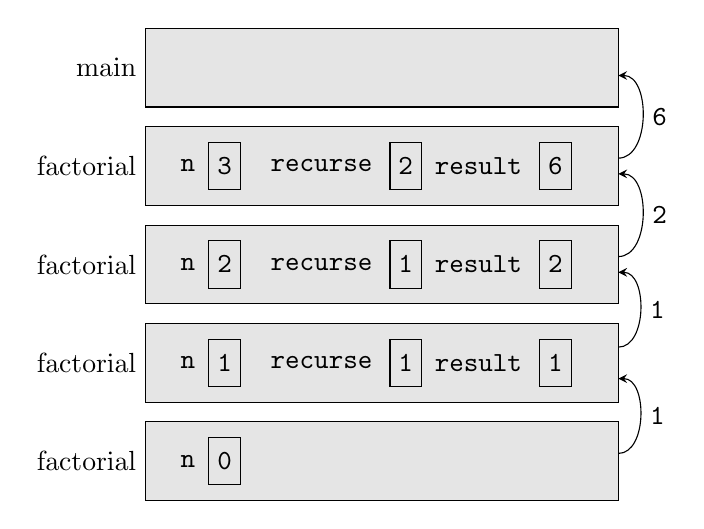
\begin{tikzpicture}
          
            \draw[fill=gray!20] (0,5) rectangle (6,6);
            \node[left] at (0,5.5) {main};
            \draw[fill=gray!20] (0,3.75) rectangle (6,4.75);
            \node[left] at (0,4.25) {factorial};
            \node[left] at (0.75,4.25) {\tt n};
            \draw (0.8,3.95) rectangle (1.2,4.55) node[pos=.5] {\tt 3};
            \node[left] at (3,4.25) {\tt recurse};
            \draw (3.1,3.95) rectangle (3.5,4.55) node[pos=.5] {\tt 2};
            \node[left] at (4.9,4.25) {\tt result};
            \draw (5,3.95) rectangle (5.4,4.55) node[pos=.5] {\tt 6};
          
            \draw[fill=gray!20] (0,2.5) rectangle (6,3.5);
            \node[left] at (0,3) {factorial};
            \node[left] at (0.75,3) {\tt n};
            \draw (0.8,2.7) rectangle (1.2,3.3) node[pos=.5] {\tt 2};
            \node[left] at (3,3) {\tt recurse};
            \draw (3.1,2.7) rectangle (3.5,3.3) node[pos=.5] {\tt 1};
            \node[left] at (4.9,3) {\tt result};
            \draw (5,2.7) rectangle (5.4,3.3) node[pos=.5] {\tt 2};
          
            \draw[fill=gray!20] (0,1.25) rectangle (6,2.25);
            \node[left] at (0,1.75) {factorial};
            \node[left] at (0.75,1.75) {\tt n};
            \draw (0.8,1.45) rectangle (1.2,2.05) node[pos=.5] {\tt 1};
            \node[left] at (3,1.75) {\tt recurse};
            \draw (3.1,1.45) rectangle (3.5,2.05) node[pos=.5] {\tt 1};
            \node[left] at (4.9,1.75) {\tt result};
            \draw (5,1.45) rectangle (5.4,2.05) node[pos=.5] {\tt 1};
          
            \draw[fill=gray!20] (0,0) rectangle (6,1);
            \node[left] at (0,0.5) {factorial};
            \node[left] at (0.75,0.5) {\tt n};
            \draw (0.8,0.2) rectangle (1.2,0.8) node[pos=.5] {\tt 0};
            
            \draw[-stealth] (6,0.6) to [out=0,in=0] node[right] {\tt 1} (6,1.55);
            \draw[-stealth] (6,1.95) to [out=0,in=0] node[right] {\tt 1} (6,2.9);
            \draw[-stealth] (6,3.1) to [out=0,in=0] node[right] {\tt 2} (6,4.15);
            \draw[-stealth] (6,4.35) to [out=0,in=0] node[right] {\tt 6} (6,5.4);
            
          \end{tikzpicture}
        \end{minipage}
        &
        \begin{minipage}{3in}
        \end{minipage}
      \end{tabular}
    \end{center}
  \begin{enumerate}
    \item Why are there no values for {\tt recurse} and {\tt result}
      in the stack diagram for the last call to {\tt factorial} (when
      \cpp{n == 0}?      
      \begin{answer}[0.5in]
        Because in that case, the function hits the base case and
        returns 1 immediately without calculating those variables.
      \end{answer}
      
    \item Looking at the stack diagram, how is it possible that the
      parameter {\tt n} can have multiple values in memory at the same
      time?
      \begin{answer}[0.5in]
        Each function call has its own separate stack frame in memory,
        so each call to {\tt factorial} has its own copy of the
        parameter {\tt n}.
      \end{answer}
  \end{enumerate}
